% This must be in the first 5 lines to tell arXiv to use pdfLaTeX, which is strongly recommended.
\pdfoutput=1
% In particular, the hyperref package requires pdfLaTeX in order to break URLs across lines.

\documentclass[11pt]{article}

\usepackage[a4paper, total={6in, 8in}]{geometry}
\usepackage{lineno}
\linenumbers

\usepackage{caption,subcaption}

\usepackage{mystyle}

\usetikzlibrary{calc,patterns,angles,quotes}    
\usetikzlibrary{decorations.pathmorphing}
\tikzset{snake it/.style={decorate, decoration=snake}}

\usepackage{natbib}
\bibliographystyle{abbrvnat}
\usepackage{hyperref}

% Standard package includes
\usepackage{times}
\usepackage{latexsym}

% For proper rendering and hyphenation of words containing Latin characters (including in bib files)
\usepackage[T1]{fontenc}
% For Vietnamese characters
% \usepackage[T5]{fontenc}
% See https://www.latex-project.org/help/documentation/encguide.pdf for other character sets

% This assumes your files are encoded as UTF8
\usepackage[utf8]{inputenc}


\title{An Application of the Implicit Function Theorem}

\author{Justin Chiu \\
  Cornell Tech \\
  \texttt{jtc257@cornell.edu}}

\begin{document}
\maketitle
\begin{abstract}
Gradient-based learning forms the foundation of modern machine learning,
and automatic differentiation allows ML practitioners to easily compute gradients.
While automatic differentiation only costs a constant multiple of the time and space
required to evaluate a function, it has its limitations.
In particular, when evaluating a function itself requires many computations,
the direct application of reverse-mode
automatic differentiation may quickly run out of memory.
In this report, we review the implicit function theorem (IFT)
and its use in reducing the cost of computing gradients in scenarios where
function evaluation is expensive,
focusing on the application of the IFT to differentiating
through the solutions of optimization problems.
\end{abstract}

\section{Introduction}
\label{sec:intro}
Gradient-based learning underpins many of the recent successes in machine learning,
particularly advances involving neural networks.
The key to the success of gradient-based methods is automatic differentiation (AD),
which greatly increases the development speed of machine learning research by
allowing practitioners to circumvent the error-prone and time-consuming process
of computing gradients manually.
AD operates by reducing functions into compositions of atomic operations,
for which we have a library of derivatives for,
and composing those derivatives via the chain rule.
The underlying concept behind AD is that a program's execution trace is a valid
and useful representation of a function \citep{griewank2008autodiff},
where the execution trace is a history of all the computation performed
during the evaluation of a program used to express a function.

Storing the execution trace of a program allows AD systems to easily compute derivatives.
However, longer execution traces can quickly consume a large amount of memory.
Consider an iterative method, such as gradient descent,
whose execution trace takes the form of an unrolled loop:
Given an initial point $\theta = x_0\in\R^n$,
iterates $x_1, x_2, ..., x_{K-1}$ and final point $x=x_K$
are produced by running the gradient descent
update for $K$ iterations, i.e. $x_{t+1} = x_{t} + \alpha \nabla f(x_t)$.
In order to differentiate through this procedure with reverse-mode AD
(i.e. compute $\frac{dx}{d\theta}$),
we have to store all the $x_k$ iterates
as well the computation used to produce them.
Thus, the memory complexity of storing this execution trace scales linearly in the
number of iterations $K$ as well as the dimensionality of the iterates $x_k$\footnote{
Forward-mode would get away from the linear dependence on $K$,
but would require $n=\dim(\theta)$ sweeps.
If all sweeps are performed in parallel,
forward-mode AD would take $\Omega(n^2)$ memory as opposed to $\Omega(Kn)$ for reverse-mode.
}.
For large $K$, this can be infeasible as the space complexity is at least $\Omega(Kn)$,
as this ignores the traces produced by the updates themselves.
One method for overcoming the space complexity's dependence on the number of iterations $K$ in
the above example is to use the implicit function theorem (IFT),
letting you throw away intermediate computation (e.g. iterates $x_1$ through $x_{K-1}$)
while still being able to compute the derivative $\frac{dx}{d\theta}$.
Naively, this comes at the cost of $O(n^2)$ space and $O(n^3)$ time,
trading off the dependence on $K$ for a larger dependence on $n$.\footnote{
This can be reduced by using approximate vector-inverse Hessian products,
as we will show later in this report.
}
We provide an illustration in Fig.~\ref{fig:optift}.

\begin{figure}
\centering
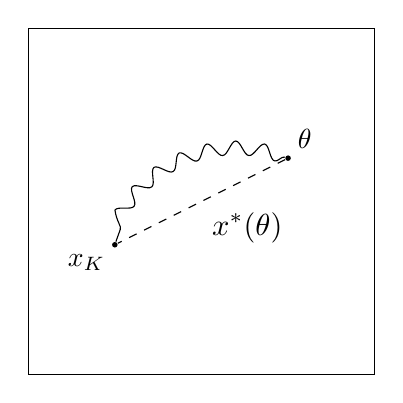
\begin{tikzpicture}[scale=1.1]
%\draw (0,0) circle (2);
\draw (-2,-2) rectangle (2,2);

\node[circle,fill=black, minimum size=2pt, inner sep=0] (x) at (1,.5) {};
\node at (x)[above right] {$\theta$};
\node[circle,fill=black, minimum size=2pt, inner sep=0] (y) at (-1,-.5) {};
\node at (y)[below left] {$x_{K}$};

\draw[snake it] (x)      to [bend right = 45] (y);
\path[dashed] (x) edge (y) node[midway,below right]{$x^*(\theta)$};

\end{tikzpicture}
\caption{
\label{fig:optift}
Reverse-mode automatic differentiation of an iterative method consumes memory
linear in the number of iterations,
illustrated by the squiggly line from initial point $\theta$ to the final point $x$.
Such methods are not uncommon, found in bilevel optimization problems such as
hyperparameter optimization and metalearning.
The implicit function theorem (IFT)
provides conditions under which there exists an implicit function,
$x^*(\theta) = x$ (dashed line), which we can use to compute the derivative
$\frac{dx_K}{d\theta}$ without storing all intermediate computation.
}
%\end{minipage}
\end{figure}


Large execution traces are not uncommon;
optimization problems are often solved with iterative methods,
resulting in traces very similar to the example given above.
In order to speed up solvers for these problems,
one could learn an initialization by differentiating through the
execution trace of the iterative method \citep{finn2017maml,kim2018savi,neuralinit}.
In this report, we will cover the use of the IFT
as a method for dealing with the space complexity of AD in exactly these cases.
In particular,
we will focus on applying the IFT to differentiating the solutions to optimization problems
\citep{optnet,agrawal2019diffcvx}.
We will walk through an example by applying the IFT to an optimization problem
that is equivalent to softmax,
then show how the approach is generalized \citep{optnet}.

\section{Related Work}
There are a variety of methods for reducing the space limitations of AD,
of which we only mention three: checkpointing, reversible computation, and implicit differentiation.

The first method, checkpointing, improves space complexity at the cost of time \citep{griewank2008autodiff}.
Rather than storing the full execution trace of a program,
checkpointing instead recomputes values when needed.
This can result in a slowdown due to recomputation,
and also requires careful choosing of which part of the trace to checkpoint and recompute.

A second method is reversible computation \citep{maclaurin2015reversible,gomez2017reversible},
which improves space complexity at the cost of expressivity, but not speed.
Reversible computation ensures that a function's derivative depends only on the output,
allowing the input to be discarded during function evaluation.
This is typically accomplished by ensuring that the input is easily reconstructed from the output,
restricting the expressivity of layers.

A third method uses the IFT, which we focus on.
Application of the IFT potentially improves space complexity at the cost of stronger assumptions.
The IFT gives conditions under which derivatives can be computed independent of
intermediate computation,
with the primary condition being the characterization of the output as the solution
to a system of equations.

One of the main applications where the space complexity of AD limits its scalability
is bilevel optimization.
Bilevel optimization problems are
optimization problems with another nested inner optimization problem embedded within.

The application we focus on in this report is expressing individual layers of a neural network declaratively
as the solution of an optimization problem \citep{optnet,agrawal2019diffcvx,gould2019declarative}.
This allows models to learn, without heavy manual specification, the constraints of the problem
in addition to the parameters of the objective.
An example of this is learning to play Sudoku from only input-output pairs \citep{optnet}.

Other applications that can be formulated as bilevel optimization problems are
hyperparameter optimization, metalearning, and variational inference.
Hyperparameter optimization formulates hyperparameter tuning as a bilevel optimization problem,
as for each hyperparameter configuration a new model must be trained as the inner loop
\citep{maclaurin2015reversible,lorraine2019implasso,lorraine2019hoift,bertrand2020implicit}.
Derivatives must then be propagated through the inner training loop to the outer hyperparameter
loop.
Similarly, metalearning learns the parameters of a model such that the model is able to quickly
be adapted to a new task via gradient descent \citep{finn2017maml,rajeswaran2019imaml}.
This is accomplished by differentiating through the learning procedure of each new task.
Finally, a variant of variational inference follows a very similar format:
semi-amortized variational inference (SAVI) aims to learn a model that is able to provide
a good initialization for variational parameters that are subsequently updated iteratively
to maximize a lower bound objective \citep{kim2018savi}.
This is also accomplished by differentiating through the iterative optimization procedure
applied to the variational parameters during inference.

In all the above applications, the inner-loop optimization problem is solved
with an iterative method, except in rare, simple cases.
The IFT reduces the memory footprint of automatic differentiation,
which would otherwise be difficult to scale.

\section{The Implicit Function Theorem}
The implicit function theorem (IFT) has a long history, as well as many applications
in a wide variety of fields such as economics and differential geometry.
For an overview of the history of the IFT and some of its classical applications
in mathematics and economics,
see the book by \citet{iftbook}.

\begin{figure}
%\begin{minipage}{0.48\textwidth}
\centering
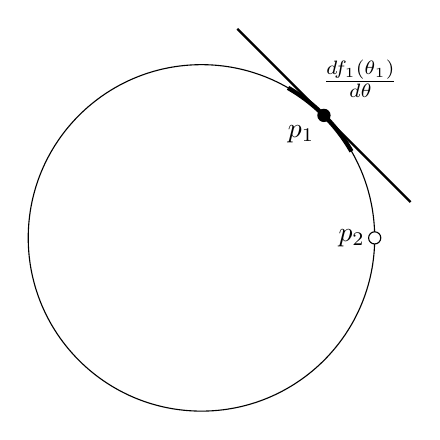
\begin{tikzpicture}[scale=1.1]
\draw (0,0) circle (2);

\node at ($2*({sqrt(2) / 2}, {sqrt(2) / 2})$) (x)[below left] {$p_1$};
\draw[fill=black] ($2*({sqrt(2) / 2}, {sqrt(2) / 2})$) circle (2pt);

% neighbourhood 
\draw[ultra thick] ($2*({sqrt(2) / 2}, {sqrt(2) / 2})$) arc(45:60:2);
\draw[ultra thick] ($2*({sqrt(2) / 2}, {sqrt(2) / 2})$) arc(45:30:2);


% tangent
%\path (2,1) node[point,label={180:P}] {P} at +(120:2){};
\node at ($2*({sqrt(2) / 2 + .21}, {sqrt(2) / 2 + .21})$) {$\frac{df_1(\theta_1)}{d\theta}$};
\draw[thick] ($2*({sqrt(2) / 2 + -.5}, {sqrt(2) / 2 + .5})$) --
    ($2*({sqrt(2) / 2 + .5}, {sqrt(2) / 2 -.5})$);

% singular point
\node at (2,0) (x2)[left] {$p_2$};
\draw[fill=white] (2,0) circle (2pt);


% axes
 
\end{tikzpicture}
\caption{
\label{fig:circle}
A circle, defined by the relation $F(\theta,x) = \theta^2 + x^2 - 1 = 0$.
We view $\theta$ as a parameter, $x$ as a solution to $F(\theta,x)=0$ given $\theta$
and the pair $(\theta,x)$ is a solution point.
Our goal is to compute the derivative $\frac{dx}{d\theta}$.
While we cannot differentiate the relation $F$ directly as it is not a function,
we can compute the derivative at the solution point $p_1 = (\theta_1,x_1)$
using the local parameterization (or solution mapping) $f_1(\theta)=\sqrt{1-x^2}$.
This parameterization holds
in a neighbourhood around $p_1$, visualized as an arc.
We can use the IFT to compute
$\frac{dx}{d\theta}= -\left[\frac{dF(\theta,x)}{dx}\right]^{-1}\frac{dF(\theta,x)}{d\theta}$,
which will agree with the derivative of the local parameterization
$\frac{df_1(\theta)}{d\theta}$.
We cannot use the same parameterization at $p_2 = (\theta_2, 0)$ as the derivative is undefined.
In general, the IFT is most useful in cases more complicated than the unit circle,
where local parameterizations are too complex to easily write down.
}
\end{figure}

Given a relation and some technical conditions that we will go over soon,
the IFT is used to identify the existence of local
function parameterizations for particular points,
and compute the Jacobians of the local function parameterizations for points
where the conditions for the IFT hold.
As a motivating example, consider the unit circle,
governed by the relation $F(\theta,x) = \theta^2 + x^2 - 1 = 0$,
which can be interpreted as a system of equations.
As $F$ fails the vertical line test, we cannot write $x$ as a function of $\theta$ globally.
This prevents us from taking derivatives, for example $\frac{dx}{d\theta}$.
However, we can use local parameterizations: $f_1(\theta) = \sqrt{1-x^2}$ if $x > 0$
or $f_2(\theta) = -\sqrt{1-x^2}$ if $x<0$.
Note that the local parameterizations are functions that hold
only within a neighbourhood of a particular solution point $(\theta,x)$;
there may be solution points where we simply cannot compute a particular derivative,
e.g. $\frac{dx}{d\theta}$ when $x=0$.
These local parameterizations then allow us compute the derivative $\frac{dx}{d\theta}$
at particular solution points $(\theta,x)$ using the corresponding parameterization.
When the conditions of the IFT do not hold a particular point,
we cannot use the IFT to ensure the existence of a local parameterization
and therefore cannot use the IFT to compute derivatives.
In general, this does not mean that the derivative does not exist,
only that the IFT does not know what it is.
See Fig.~\ref{fig:circle} for an illustration.
The IFT generalizes this example, and formalizes the conditions under which there exist
continuous local parameterizations for a given relation or system of equations.

While the unit circle in this example has very simple local parameterizations,
in general local parameterizations can be more complicated.\footnote{
Recall that a program trace is a valid representation of a function.
One could have a local parameterization that is the trace of a long program,
such as one that consists of a series of iterative updates.
}
Additionally, the IFT does not give the form of the local parameterizations;
it only guarantees the existence of one around a point and a way to compute its derivative.
The local parameterization is left implicit, hence the `implicit' in IFT.

Formally, given a system of equations $F(\theta, x) = \mathbf{0}_m$,\footnote{
We denote vectors and matrices of all 1s and 0s by $\mathbf{1}_S$
and $\mathbf{0}_S$, where $S$ denotes the shape, i.e. $\mathbf{0}_m\in\R^m$.
}
and a solution point $(\theta,x) \in \R^n\times\R^m$,
the IFT gives sufficient conditions under which $x$ can locally be written as a function
of just the parameters $\theta$ within a neighbourhood of the solution point $(\theta,x)$.
We saw this in the unit circle example, where the local parameterizations were
valid around a particular solution point.
We refer to this function $x^*(\theta) = x$ as a solution mapping,
$x$ a solution, and $\theta$ as parameters.
These conditions are as follows:
\begin{enumerate}
\item We have a solution point $(\theta, x)$ that satisfies the system of equations
    $F(\theta, x) = 0$.
\item $F$ has at least continuous first derivatives: $F \in \mcC^1$.
\item The Jacobian matrix
    of $F$ wrt $x$ evaluated at the solution point $(\theta,x)$ is nonsingular:
    $\det \frac{d F(\theta,x)}{d x} \neq 0$.
\end{enumerate}
Assuming these conditions hold for $F$ at $(\theta,x)$, the IFT
asserts the existence of the implicit solution mapping $x^*(\theta):\R^n\to\R^m$
(at the solution point $(\theta,x)$),
and that the derivative of the solution mapping wrt the parameters is given by
\begin{equation}
    \label{eqn:iftderiv}
    \frac{d x^*(\theta)}{d\theta} = -\left[\frac{dF(\theta,x)}{dx}\right]^{-1}
    \frac{d F(\theta,x)}{d\theta} \in \R^{m\times n}.
\end{equation}
As long as we have chosen a solution point $(\theta,x)$ that satisfies the conditions,
we can ignore how we arrived at that solution point and still compute the derivative
of the solution mapping with the IFT.
It is important to note that the IFT is local and applies to particular solution points.
This means that we can pick and choose which solution points we restrict our analysis to.

\paragraph{Notation: Jacobian Matrix}
Given a function $F:\R^n\times\R^m\to\R^m$, we denote the Jacobian matrix evaluated at
the point $(\theta,x)\in\R^n\times\R^m$ as
\begin{equation*}
\frac{dF(\theta,x)}{d(\theta,x)} = \begin{bmatrix}
    \frac{dF(\theta,x)}{d\theta} &\frac{dF(\theta,x)}{dx} 
\end{bmatrix},
\end{equation*}
where we have the matrix of partial derivatives
\begin{equation*}
\frac{dF(\theta,x)}{d\theta} = \begin{bmatrix}
    \frac{dF_1(\theta,x)}{d\theta_1} & \cdots & \frac{dF_1(\theta,x)}{d\theta_n} \\
    \vdots & \ddots & \vdots \\
    \frac{dF_m(\theta,x)}{d\theta_1} & \cdots & \frac{dF_m(\theta,x)}{d\theta_n} \\
\end{bmatrix}\in\R^{m\times n},
\end{equation*}
and similarly for $\frac{dF(\theta,x)}{dx}\in\R^{m\times m}$.

%{\color{red} still searching for a good intuitive explanation.}

Given the IFT and necessary notation, we can now proceed to use the IFT
to compute derivatives of the output of an iterative method,
as depicted in Fig.~\ref{fig:optift}.
In particular, we focus on computing derivatives of the solution to a
constrained optimization problem.
We will use the optimality criteria of the optimization problem to define a system of equations,
then apply the IFT to compute the Jacobian of the solution wrt the parameters.
This methodology allows us to use the solution to an optimization problem
as the output of a layer within a neural network,
as done in OptNet \citep{optnet}.
%We will then discuss the problem addressed by this method in OptNet.

%Afterwards, we will cover an application of the IFT to speeding up variational inference.

\section{Differentiating through Optimization}
As an introductory example,
we will replace softmax with an equivalent function
defined as the output of an optimization problem, then derive derivatives using the IFT.
We will start by reviewing softmax and its expression as an optimization problem.
After checking the conditions of the IFT hold, we can then compute derivatives.
Since the Jacobian of softmax is known, we can directly verify that the IFT gives
the correct answer.

\subsection{Softmax}
Softmax is often used to parameterize categorical distributions within neural networks,
such as in attention layers.
Given $n$ items with independent utilities, where $\theta \in \R^n$
indicate preferences,
softmax gives the following distribution over items:
$z_i = \softmax(\theta)_i = \frac{\exp(\theta_i)}{\sum_j \exp(\theta_j)}$, with $z\in[0,1]^n$.
While there is a closed-form equation
for both softmax and its Jacobian,
we use it as an introduction to the mechanism
behind OptNet (and other differentiable optimization layers)
\citep{optnet,agrawal2019diffcvx}.

The output of softmax is the solution of the following constrained optimization problem
\citep{gao2018properties}:
\begin{equation}
\label{eqn:softmax-opt}
\begin{aligned}
\textrm{maximize } \quad & z^\top\theta + H(z)\\
\textrm{subject to } \quad & z^\top \mathbf{1} = 1\\
& z_i \geq 0, \forall i,
\end{aligned}
\end{equation}
where $H(z) = -\sum_i z_i \log z_i$ is the entropy.
The first term in the objective, $z^\top\theta$, is highest when $z$ points in the
same direction as $\theta$.
Given the constraint that $z$ must sum to one and have nonnegative entries,
maximizing just the first term subject to those constraints results in a solution
that picks out the highest component of $\theta$, i.e. $\argmax(\theta)$.
The addition of the entropy term penalizes solutions that put too much
mass on just a few items, resulting in a smoothed version of argmax.
We will refer to this entropy-regularized version as the softmax problem.\footnote{
Removing the entropy regularization term results in the argmax optimization problem:
maximize $z^\top\theta$, subject to $z^\top\mathbf{1}_n=1$
and $z \succeq 0$.
This is known as the support function of the set $\set{z\mid z^\top\mathbf{1}_n=1,z\succeq 0}$.
}

Our goal is to compute the Jacobian of softmax
$\frac{dz}{d\theta} = \frac{d\softmax(\theta)}{d\theta}$
using the IFT and the optimization problem above.
While this may seem trivial because softmax has a closed form expression for
both the output and Jacobian, it is a worthwhile exercise in applying the IFT.
Applying the IFT to optimization problems consists of four steps:
\begin{enumerate}
\item Find a solution to the optimization problem.
\item Write down a system of equations derived from the optimality conditions.
\item Check that the conditions of the IFT hold.
\item Compute the derivative of the implicit solution mapping wrt the parameters.
\end{enumerate}

We assume the first step has been done for us,
and we have a solution $z$ to the softmax problem.\footnote{
This is trivial for softmax since we can compute it using the closed form
expression.
However, in more general optimization problems, we would obtain $z$ from a solver
with a large execution trace.}
We will then use the IFT to compute gradients of $z$ wrt the parameters $\theta$
by following the rest of the steps.

\subsection*{Step 2: The KKT conditions determine the system of equations}
In order to apply the IFT,
we need a system of equations for which our outputs of interest are solution points for.
The goal of this step is to choose a suitable system of equations.
This differs from the example of the unit-circle, which was already defined by
a system of equations.\footnote{
For a given solution point there may be many suitable systems,
all of which would be viable as long as they satisfy
the conditions of the IFT that we will check in step 3.
}

For solutions of optimization problems, the Karush-Kuhn-Tucker (KKT) conditions
are a natural choice for defining such a system of equations.
Given an optimization problem, the KKT conditions
determine a system of equations that the solution must satisfy
based on the optimality criteria \citep{kkt-thesis,kkt}.
They are stationarity (the gradient should be 0 at a local optima)
and feasibility (the constraints of the problem should not be violated).
For a thorough introduction to the KKT conditions, see chapter 5 of \citet{bv-cvxbook}
or the \href{https://en.wikipedia.org/wiki/Karush-Kuhn-Tucker\_conditions}{Wikipedia article}

We will use the KKT conditions of the softmax problem in
Eqn.~\ref{eqn:softmax-opt} to determine the (vector-valued) function $F:\R^n\times\R^m\to\R^m$
in the IFT.
First, we introduce dual variables $u\in\R,v\in\R^n$ and write out the Lagrangian:
$$\mcL(\theta, z, u, v) = z^\top\theta + H(z) + u(z^\top \mathbf{1}_n - 1) + v^\top z.$$
We therefore have the solution point $(\theta,z,u,v)$, with parameters $\theta$
and solution $x=(z,u,v)$.
We then have the following necessary conditions for a solution $(z,u,v)$,
i.e. the KKT conditions:
\begin{equation}
\begin{aligned}
\frac{d}{dx} \mcL(\theta, z,u,v) &= \mathbf{0}_n && \textrm{(stationarity)}\\
u(z^{\top} \mathbf{1} - 1) &= 0 && \textrm{(primal feasibility, equality)}\\
\diag(v)z &= \mathbf{0}_{n} && \textrm{(complementary slackness)}\\
z &\succeq \mathbf{0}_n && \textrm{(primal feasibility, inequality)}\\
v &\succeq \mathbf{0}_n && \textrm{(dual feasibility)}
\end{aligned}
\end{equation}
As we only need a system of equations with $2n+1$ equations to
determine the $2n+1$ solution variables $x=(z,u,v)$,
we use the first three conditions: stationary, primal feasibility (equality),
and complementary slackness.

In full, the system of equations $F(\theta, z,u,v) = 0$ we choose
for the softmax problem is
\begin{equation}
\label{eqn:system}
\begin{aligned}
\theta + -\log(z) - 1 + u\mathbf{1}_n + v &= \mathbf{0}_n\\
u(z^{\top} \mathbf{1}_n - 1) &= 0\\
\diag(v)z &= \mathbf{0}_n.
\end{aligned}
\end{equation}
Note that the first and third equations are vector-valued.

This completes the second step, where we chose a subset of the KKT conditions
in order to produce a nonlinear system of equations.
We can now proceed check the conditions of the IFT,
which will determine whether $F$ is locally well-behaved
at a particular solution point $(\theta, z,u,v)$.

\subsection*{Step 3: Check that the IFT conditions hold at the solution point}
Recall that the IFT requires the following three conditions,
which must be checked on a case-by-case basis for particular
solution points\footnote{If these conditions do not hold,
the IFT does not apply at this particular combination of $F$ and solution point.
The derivative $\frac{dx}{d\theta}$ may still be computed via other means
if it exists.}:
\begin{itemize}
    \item $F(\theta,z,u,v) = 0$,
    \item $F$ has at least continuous first derivatives,
    \item $\det\frac{dF(\theta,z,u,v)}{d(z,u,v)} \ne 0$,
        or equivalently $\frac{dF(\theta,z,u,v)}{d(z,u,v)}$
        is full rank.
\end{itemize}
Returning to the softmax problem,
the first condition holds as we have a solution to the optimization problem
and $F$ was chosen using the KKT conditions.\footnote{
Recall that softmax also has a closed form expression.}
The second condition also holds, as $F$ has continuous first derivatives.
All that remains is to check the third condition,
that the Jacobian matrix $\frac{dF(\theta,z,u,v)}{d(z,u,v)}$
(evaluated at the solution point) is non-singular.

The Jacobian matrix $\frac{dF(\theta,z,u,v)}{d(z,u,v)}\in\R^{2n+1\times 2n+1}$ is given by
\begin{equation}
\label{eqn:f-jac}
\frac{dF}{d(z,u,v)}=
\begin{bmatrix}
\diag(z)^{-1} & -\mathbf{1}_n & -I_{n\times n} \\
u\mathbf{1}_n^\top & z^\top\mathbf{1}_n - 1 & 0\\
\diag(v) & 0 & \diag(z)
\end{bmatrix}.
\end{equation}
Since a solution must be feasible, we know that $z^\top\mathbf{1}-1=0$ and $u > 0$.
However, the upper left block, $\diag(z)^{-1}$, contains a divide-by-zero term if
any component $z_i = 0$.\footnote{
This term was obtained by differentiating the entropy
term of the Lagrangian, $H(z) = \sum_i z_i\log z_i$.
While we could use the convention $0\log 0 = 0$,
this does not fix the divide-by-zero issue with the second derivative, which we see here.
}
To avoid this, we consider only strictly positive $z \succ 0$ for the IFT.\footnote{
We saw a similar issue in the unit circle example, where the derivative
$\frac{dx}{d\theta}$ was undefined when $x=0$ (see Fig.~\ref{fig:circle}).
}
Constraining to strict positivity for $z$,
we can deduce that the Jacobian of $F$ is full rank and therefore has nonzero determinant.
This shows that the conditions of the IFT hold for the solution points that are
feasible, optimal, and have strictly positive $z$.\footnote{
Recall that the IFT applies at particular solution points,
meaning we can pick and choose which points to analyze.
In the case of softmax, we can perform a separate analysis
for solution points on the boundary of the constraint set.
}

\subsection*{Step 4: Compute $\frac{dx}{d\theta}$}
Now that we have a set of solution points where conditions of the IFT hold,
we can use the IFT to compute $\frac{dz}{d\theta}$.
Recall that we have the solution $x = (z,u,v)$; we will switch to $x$ for brevity.
The second part of the IFT (Eqn.~\ref{eqn:iftderiv})
tells us that we can compute the Jacobian of the
solution mapping $\frac{dx}{d\theta} = \frac{dx^*(\theta)}{d\theta}
= -\left[\frac{dF(\theta,x)}{dx}\right]^{-1}\frac{dF(\theta,x)}{d\theta}$,
then pick out the relevant components.

The second term, $\frac{dF(\theta,x)}{d\theta}$, is simple.
Since $\theta$ only appears in the first vector-valued function of $F$
(see Eqn.~\ref{eqn:system}), we have
\begin{equation}
\label{eqn:df-dtheta}
\frac{dF(\theta,x)}{d\theta} = \begin{bmatrix}
    I_{n\times n}\\
    \mathbf{0}_{(n+1)\times (n+1)}
\end{bmatrix}.
\end{equation}
The large amount of sparsity allows us to skip some computation further down.

Next, we have to invert the Jacobian from Eqn.~\ref{eqn:f-jac}:
\begin{equation}
\label{eqn:dsystem-matrix}
\left[\frac{dF(\theta,x)}{dx}\right]^{-1} = \begin{bmatrix}
\diag(z)^{-1} & -\mathbf{1}_n & -I_{n\times n} \\
u\mathbf{1}_n^\top & x^\top\mathbf{1}_n - 1 & 0\\
\diag(v) & 0 & \diag(z)
\end{bmatrix}^{-1}.
\end{equation}
The remainder of this section is compute-intensive;
feel free to skip ahead to Sec.~\ref{sec:limitations} for a discussion
on the limitations of applying the IFT.
We use the block-wise inversion formula
\begin{equation*}
\begin{bmatrix}
A & B\\
C & D
\end{bmatrix}^{-1} = \begin{bmatrix}
    (A - BD^{-1}C)^{-1} & 0\\
    0 & (D - CA^{-1}B)^{-1}
\end{bmatrix}
\begin{bmatrix}
    I & -BD^{-1}\\
    -CA^{-1} & I
\end{bmatrix},
\end{equation*}
where
\begin{align*}
A = \begin{bmatrix} \diag(z)^{-1} & -\mathbf{1}_n \\ u\mathbf{1}_n^\top & 0 \end{bmatrix}&\qquad\qquad
B = \begin{bmatrix}-I_{n\times n} \\ 0\end{bmatrix}\\
C = \begin{bmatrix}\diag(v) & 0\end{bmatrix} &\qquad\qquad
D = \diag(z).
\end{align*}
However, by complementary slackness, we have $v = 0$,\footnote{
We apply the IFT to solutions where $z\succ 0$ due to a divide-by-zero issue
in $\frac{d^2H(z)}{dz_i^2} = \frac{1}{z_i}$.
}
reducing the above to
\begin{equation*}
\begin{bmatrix}
A & B\\
C & D
\end{bmatrix}^{-1} = \begin{bmatrix}
    A^{-1} & 0\\
    0 & D^{-1}
\end{bmatrix}
\begin{bmatrix}
    I_{(n+1)\times (n+1)} & -BD^{-1}\\
    0 & I_{n \times n}
\end{bmatrix}.
\end{equation*}
As we are interested in computing $\frac{dz}{d\theta}$,
rather than the full derivative $\frac{dx}{d\theta}$ (recall $x = (z,u,v)$),
in addition to the sparsity of $\frac{dF}{d\theta}$, 
we only have to solve for the upper-left $n\times n$ block of $A^{-1}\in\R^{n+1\times n+1}$.
To do so, we will repeat the same block-wise inverse computation.
Let us denote
$$A
= \begin{bmatrix} \diag(z)^{-1} & -\mathbf{1}_n \\ u\mathbf{1}_n^\top & 0 \end{bmatrix}
= \begin{bmatrix}E & F \\ G & H\end{bmatrix}.
$$
First, we compute the Schur complement of $A$,
\begin{equation}
A/E = H - GE^{-1}F = 0 + u\mathbf{1}_n^\top\diag(z)\mathbf{1}_n = uz^\top\mathbf{1}_n.
\end{equation}
Since $z$ is feasible, we have $A/E = u$ due to the equality constraints
($z$ must sum to 1 as a probability mass function).
Then, we have
\begin{equation}
A^{-1} = \begin{bmatrix}
\diag(z)^{-1} & -\mathbf{1}_n\\
u\mathbf{1}^\top_n & 0
\end{bmatrix}^{-1}
=\begin{bmatrix}E & F \\ G & H\end{bmatrix}^{-1}
= \begin{bmatrix}
E^{-1} + E^{-1}F(A/E)^{-1}GE^{-1} & -E^{-1}F(A/E)^{-1}\\
-(A/E)^{-1}GE^{-1} & (A/E)^{-1}
\end{bmatrix}.
\end{equation}
Plugging in,
\begin{equation}
\begin{aligned}
A^{-1} 
&= \begin{bmatrix}
\diag(z) - \diag(z)\mathbf{1}_nu^{-1}u\mathbf{1}^\top_n\diag(z)
    & \diag(z)\mathbf{1}_nu^{-1}\\
-u^{-1}u\mathbf{1}^\top_n \diag(z) & u^{-1}
\end{bmatrix}\\
&= \begin{bmatrix}
\diag(z) - zz^\top
    & u^{-1}z\\
    -z^\top & u^{-1}
\end{bmatrix}.
\end{aligned}
\end{equation}
Pulling out the top-left $n\times n$ block yields
the Jacobian $\frac{d z}{d\theta} = \diag(z) - zz^\top$,
which agrees with directly differentiating softmax \citep{sparsemax}.
While we were able to take advantage of sparsity in this computation,
such sparsity may not be available in general.
Without sparsity, inverting the Jacobian of $F$, $\frac{dF(\theta,x)}{dx}$,
costs $O(n^3)$ time and $O(n^2)$ space
compared to the $O(n)$ time and space for computing softmax and its
derivative exactly (as well as with the IFT and sparsity).

This concludes the exercise of using the IFT to differentiate through the
softmax problem.
While softmax itself has a closed form expression for both its output and derivative,
we showed that the IFT can also be used to compute its derivative in a solver-agnostic manner.
We started by expressing softmax as an optimization problem (Eqn.~\ref{eqn:softmax-opt}),
then, assuming we had a solution to the softmax problem (regardless of how it was obtained),
reverse engineered a system of equations using the KKT conditions.
We then restricted our attention to the set of solution points where we could succssfully
apply the IFT,
then applied Eqn.~\ref{eqn:iftderiv} to compute the derivative at a solution point.

%(Example showing build-up of memory from reversible SGD vs IFT would be nice here,
%ie code it up and plot memory consumption / speed. maybe not best example though)

\subsection{Limitations}
\label{sec:limitations}
In order to compute the derivative $\frac{dx}{d\theta}$, we had to invert the Jacobian of $F$
(the system of equations derived from the KKT conditions),
i.e. compute $\left[\frac{dF(\theta,x)}{dx}\right]^{-1}$.
However, the first part of $F$ (recall from Eqn.~\ref{eqn:system}), the stationarity condition
$\frac{d}{dx}\mcL = 0$
already involved the Jacobian of the Lagrangian $\mcL$.
In general, this means that in order to apply the IFT to solutions of optimization problems,
we must compute the inverse Hessian of the Lagrangian (or at least an inverse Hessian-vector-product).
The Hessian is a matrix of size $O(n^2)$,
and inverting this would take $O(n^3)$ computation.\footnote{
The number of solution variables scales with the number of primal variables,
but also the number of constraints.
This potentially makes applying the IFT to optimization problems with exponentially
many constraints difficult.
}
Thankfully, there are relatively cheap ways of approximating this computation,
such as with approximate (inverse) Hessian-vector-product techniques
\citep{rajeswaran2019imaml,lorraine2019hoift}.

\subsection{Extensions}
The methods we covered can be extended to variations of argmax problems
other than the softmax problem.\footnote{
The argmax problem is given by maximize $z^\top \theta$, subject to $z^\top\mathbf{1}_n=1$
and $z\succeq 0$.
}
The softmax problem altered the argmax problem by introducing entropy regularization.
Rather than regularizing with entropy, one could instead alter the objective to find
the Euclidean projection of the parameters onto the probability simplex,
resulting in SparseMax \citep{sparsemax}.
While the output of softmax variants often have a closed form expression,
the IFT provides another way of deriving their Jacobians
and could potentially pave the way for differentiating through argmax problems
that do not have closed-form expressions.

More generally, the IFT can be applied to cases where, unlike softmax,
we do not have an explicit functional form (i.e., the unit circle),
and outputs are governed only by a system of equations.
This includes more general optimization problems, such as quadratic programs \citep{optnet}
or other convex optimization problems \citep{agrawal2019diffcvx}.
%as well as the solutions of differential equations \citep{neuralode}.

\section{OptNet}
OptNet generalizes the methodology applied above to the softmax problem by
extending the optimization problems considered,
in particular including parameterized constraints.
This allows us to learn not only the objective, but also the constraints.
Explicitly incorporating families of constraints in models
with optimization layers to allows them to perform well
on tasks with rigid constraints, such as learning to play
Sudoku from only inputs and outputs \citep{optnet}.

OptNet applies the IFT to quadratic programs (QPs) in particular.
As the simplest nonlinear optimization problem,
QPs strike a balance between expressivity and computational tractability \citep{simplex}.
The methodology remains the same as the softmax problem:
Given a QP and a solution,
use the KKT conditions to produce a system of equations then apply the IFT
to compute the derivative of the solution wrt the
parameters of the objective and constraints.

Quadratic programs take the following form:
\begin{equation}
\label{eqn:qp}
\begin{aligned}
\textrm{minimize } \quad & \frac12 z^\top Q z + q^\top z\\
\textrm{subject to } \quad
& Gz \leq h\\
& Az = b,
\end{aligned}
\end{equation}
where we optimize over $z\in\R^n$ and the parameters are $\theta = \set{Q, q, A, b, G, h}$,
with $Q\in\R^{n\times n}\succeq0, q\in\R^n, A\in\R^{m\times n},b\in\R^{m},G\in\R^{p\times n},
h\in\R^p$.
Compared to the softmax problem in Eqn.~\ref{eqn:softmax-opt},
the main difference is the learnable parameters in the constraints.
As the application of the IFT is very similar, we will not cover it in as much
detail as the softmax problem.

Similar to the softmax problem, we will first assume we already have a solution.
Unlike in the softmax problem, we assume the the solution to the QP is provided by a solver,
as there may not be a closed-form solution.\footnote{
One contribution of OptNet was the extension of a state-of-the-art interior point
solver \citep{optnet}, and its adaptation to parallel machines (GPUs) and batch processing.
While outside the scope of this report, see the paper by \citet{optnet} for the details.
}
In this case, the execution trace of the solver may be too large to store in memory,
necessitating the use of the IFT.

\subsection*{Step 2: The KKT conditions determine the system of equations}
The Lagrangian of the QP is given by
$$
\mcL(\theta,z,u,v) = \frac12 z^\top Qz + q^\top z + u^\top(Gz-h) + v^\top(Az-b),
$$
introducing dual variables $u\in\R^p,v\in\R^m$,
where we have the solution $x = (z,u,v)$.

We use the following subset of the KKT conditions to determine our system of equations:
stationarity, primal feasibility (equality), and complementary slackness.
This yields, written in full,
\begin{equation}
\begin{aligned}
Qz + q + G^\top u + A^\top v  &= \mathbf{0}_n\\
\diag(u)(Gz-h) &= \mathbf{0}_p\\
\diag(v)(Az-b) &= \mathbf{0}_m.
\end{aligned}
\end{equation}

\subsection*{Step 3: Check the conditions of the IFT}
As with the softmax problem,
the only nontrivial part is checking that the Jacobian matrix of $\frac{dF(\theta,x)}{dx}$ is
not singular at the solution point(s) of interest $(\theta,x)$.
This computation is more involved for QPs than the softmax problem. 
See Theorem 1 and its proof in the OptNet paper for more details \citep{optnet}.

\subsection*{Step 4: Compute $\frac{dx}{d\theta}$}
We would then compute
$\frac{dx}{d\theta} = \left[\frac{dF(\theta,x)}{dx}\right]^{-1}\frac{dF(\theta,x)}{d\theta}$
by hand or numerically.
\citet{optnet} also show how to obtain the vector-Jacobian product efficiently
using quantities readily available from a QP solver.

\section{Gradient Estimation in Hidden Markov Models}
We now apply the IFT to structured latent variable models.
Similar to the softmax case, we can compute both the solution and gradient
exactly without using too much memory.
In the case of hidden Markov models (HMMs), we can perform inference in time linear
in the length of a sequence and quadratic in the number of states and
space linear in length and the number of states.



\section{Variational Inference}
Variational inference has found success in recent applications to generative models,
in particular by allowing practitioners to depart from conjugate models
and extend emission models with expressive neural network components.
The main insight that led to this development is that inference can be amortized through
the use of an inference network.
One approach to variational inference, stochastic variational inference (SVI),
introduces local, independent variational parameters for every instance of hidden variable.
While flexible, the storage of all variational parameters is expensive, and the optimization
of each parameter independently slow \citep{}.
Amortized variational inference (AVI) solves that by instead using a hierarchical process.
Variational parameters are produced hierarchically via an inference network,
which in turn generates the local variational parameters \citep{}.
The resulting local parameters may or may not be subsequently optimized.

Failure to further optimize local variational parameters may result in an amortization gap \citep{}.
Prior work has shown that this gap can be ameliorated by performing a few steps of
optimization on the generated local parameters obtained from the inference network,
and even by propagating gradients through the optimization process.
Optimizing through the inner optimization problem results in semi-amortized variational inference
(SAVI) \citep{}.

As our main motivating example, we will examine whether we can apply the IFT to SAVI.
We will start by formalizing the problem of variational inference for a simple model.

We will start with a model defined by the following generative process,
used by \citet{dai2020vae} to analyze posterior collapse:
\begin{enumerate}
\item Choose a latent code from the prior distribution $z \sim p(z) = N(0, I)$.
\item Given the code, choose an observation from the emission distribution
    $x \mid z \sim p_\theta(x \mid z) = N(\mu_x(z, \theta), \gamma I)$,
\end{enumerate}
where $\mu_x(z, \theta) \equiv \MLP(z, \theta)$ and $\gamma > 0$ is a hyperparameter.
This yields the joint distribution $p(x,z) = p(x\mid z)p(z)$.

Since the latent code $z$ is unobserved, training this model would require optimizing the
evidence $p(x) = \int p(x,z)$.
However, due to the MLP parameterized $\mu_x$, the integral is intractable.
Variational inference performs approximate inference by introducing variational distribution
$q_\phi(z \mid x)$ and maximizing the following lower bound on $\log p(x)$:
\begin{equation}
    \log p(x) - \KL{q(z \mid x) || p(z \mid x)}
    = \Es{q_\phi(z \mid x)}{\log \frac{p_\theta(x,z)}{q_\phi(z\mid x)}} = L(\theta, \phi).
\end{equation}

(Write out objective in full.)

While SVI introduces local parameters for each instance of $z$,
and AVI uses a single $q(z \mid x)$ for all instances,
we will follow the approach of SAVI.
We will perform inference as follows:
For each instance $x$, produce local variational parameter
$z^{(0)} = g(x; \phi)$.
Obtain $z^*$ by solving $\mcL(\theta, z^{(0)}) = 2$, with (local) optima $\ell^*$.
Take gradients through the whole procedure,
i.e. compute $\frac{\partial \ell^*}{\partial \phi}
= \frac{\partial\ell^*}{\partial z^*}\frac{\partial z^*}{\partial z^{(0)}}
\frac{\partial z^{(0)}}{\partial \lambda}$.
The main difficuty lies in computing $\frac{\partial z^*}{\partial z^{(0)}}$.
(Highlight challenge)

In order to avoid the memory costs of storing all intermediate computation performed
in a solver, we will instead apply the IFT.
In order to apply the IFT, we must satisfy the three conditions.
First, we must have a solution point to a system of equations, $F(x_0, z_0) = 0$.
In this setting, we will use the KKT conditions of the optimization problem to define $F$.

\section{Limitations}

\bibliography{bib}

\appendix

\section{Properties of Exponential Family Distributions}
\label{sec:exp-fam}
Exponential family distributions are widely used to parameterize graphical models \citep{vi}.
The classification of a distribution as exponential family simply says that we can write
their joint distributions with the particular factorization given above,
which can then be used to derive useful properties common to all exponential
family distributions.
These properties, made clearer through the exponential family abstraction,
are then integral for performing inference.
In particular, gradient estimation can be written as mapping from
canonical to mean parameters.

\subsection{Canonical Parameters}
Exponential family distributions take the form
\begin{equation}
    \label{eqn:exp-canon}
    p(x;\theta) = h(x)\exp(\theta^\top \phi(x)-A(\theta)),
\end{equation}
where $h:\mcX\to\R_+$ is the base measure,
$\theta\in\R^d$ the canonical parameters,
$\phi:\mcX\to\R^d$ the sufficient statistics\footnote{Potential functions usually refer to
particular pairs of canonical parameter and sufficient statistic products
$\theta_\alpha\phi_alpha(x)$ as a function of $x$.},
and $A:\R^d\to\R$ the log partition function.
Intuitively, the canonical parameters $\theta$ score configurations $x\in\mcX$,
with representation $\phi(x)$.
The log partition function $A(\theta) = \log\int_{\mcX}h(x)\exp(\theta^\top\phi(x))$
is used to ensure normaliziation of the probability density,
i.e. $\int_{\mcX}p(x) = 1$.
The base measure $h:\mcX\to\R$ is also used to ensure proper normalization,
but is only a function of $x$.
It can also be used to enforce hard constraints in models by giving
0 mass to some configurations $x$.

We give three examples of exponential family distributions:
softmax, hidden Markov models (HMMs)
and linear chain conditional random fields (CRFs).

\paragraph{Softmax}
Softmax gives a discrete distribution over $n$ items, where $x\in[1,\ldots,n]$.
The probability mass function is then $p(x;\theta) = \exp(\theta^\top x - A(\theta))$,
where $A(\theta) = \log \sum_i \exp(\theta_i) = \log \exp(\theta)^\top\mathbf{1}_n$.
Thus, the sufficient statistics are $\phi(x)_i = 1(x_i)$ for each $i\in[n]$ and
the base measure constant $h(x)=1$.

\paragraph{Hidden Markov Models (HMMs)}
Hidden Markov models (HMMs) give a discrete distribution over sequences $x = (x_1,\ldots,x_T)$,
where $x_t\in[X]$,
and latent states $z = (z_1,\ldots,z_T)$, where $z_t\in[Z]$.
HMMs have the joint distribution
$p(x,z) = \prod_t p(x_t\mid z_t)p(z_t\mid z_{t-1})$,
with distinct start state $z_0=\epsilon$.
We assume each condition distribution is parameterized using softmax,
and the HMM has canonical parameters $\theta = (O,S)$ for the emission and transitions respectively.
The emissions are locally normalized, given by $p(x_t\mid z_t) = O 1_{z_t,x_t}$
where $O\in[0,1]^{ZX}$, $1_{z_t,x_t}\in\R^{ZX}$ is a one-hot vector.
Local normalization implies $\sum_x O_{z,x}=1$ for a given $z$.
The transitions are also locally normalized, given by $p(z_t\mid z_{t-1}) = S 1_{z_{t-1},z_t}$,
where $S\in[0,1]^{Z^2}$, $1_{z_{t-1},z_t}\in\set{0,1}^{Z^2}$ is a one-hot vector.
Both $O$ and $S$ are vector representations of the observation and state transition
matrices respectively.
The sufficient statistics are $\set{1(x_t,z_t)}_{x_t,z_t}$
and $\set{1(z_{t-1}),1(z_t)}_{z_{t-1},z_t}$ for all $t,x_t,z_{t-1},z_t$.
The base measure is constant $h(x,z) = 1$.

\paragraph{Linear Chain Conditional Random Fields (CRFs)}
The linear chain CRF has states $x = (x_1,\ldots,x_T)$, where $x_t\in[Z]$,
and joint distribution
$$p(x) = \frac{\prod_t f(z_t; \theta)g(z_{t-1},z_t; \theta)}{\exp(A(\theta))}
= \exp(\theta^\top \phi(x) - A(\theta)),$$
where $f:\mcX\to\R_+,g:\mcX\times\mcX\to\R_+$ are unary and binary potentials respectively.
These potentials are the most common representation of CRFs.
In the exponential family representation,
the canonical parameters $\theta\in\R^{(Z + Z^2)T}$ are used to score unary and binary terms,
given by the sufficient statistics $\phi(x)_{t,1,i} = 1(z_t = i)$ and
$\phi(x)_{t,2,ij} = 1(z_{t-1} = i, z_t = j)$ for $t,i,j$.
The base measure is constant $h(x) = 1$.

\subsection{Mean Parameters}
The mean parameters of exponential family distributions are the expected sufficient statistics:
$\mu = \Es{p(x)}{\phi(x)}$.
The space of all possible marginals, obtained by varying the distribution
$p(x)$, is called the mean parameter space
$$\mcM = \set{\mu \mid \exists p \textrm{ s.t. } \Es{p}{\phi(x)} = \mu}.$$
For the particular case of discrete graphical models,
which is of particular interest,
we call $\mcM$ the marginal polytope.
In particular, for discrete models, we have
$$\mcM = \set{\mu | \sum_x p(x)\phi(x) = \mu, \sum_x p(x) = 1},$$
expressed as a finitely generated polyhedra.
By the Minkowski-Weyl theorem, we can equivalently express the marginal polytope
as a constrained polyhedra, i.e. the convex hull of the sufficient statistics:
$$\mcM = \conv(\phi(x),x\in\mcX).$$
This representation is more useful in variational optimization problems,
as it translates directly to a set of constraints.

\subsection{Forward and Backward Mappings from Canonical to Mean Parameters}
The forward mapping $\theta\mapsto\mu$ is marginal inference in CRFs,
while the backward mapping $\mu\mapsto\theta$ corresponds to learning.
The log partition function $A(\theta)$ is key to both of these mappings:
\begin{itemize}
\item[Forward] $\nabla A(\theta) = \mu$
\item[Backward] $\theta \in \nabla A^*(\mu)$
\end{itemize}
where $A^*(\mu)$ denotes the conjugate dual function of $A$.
When the mean parameters are in the interior of the mean parameter space
(henceforth referred to as the marginal polytope, as we focus on discrete
graphical models)
$\mu\in\mcM^{\circ}$,
the conjugate dual function $A^*(\mu) = -H(p_{\theta(\mu)})$
{\color{red} More precise definition following \citet{vi} Thm. 3.4}.


\section{Graphical Models}

Neural ODEs use reversibility.

\end{document}
